\chapter{Methodology}
\label{ch:methodology}

In this chapter we discuss the methods and techniques used for both the machine learning and background subtraction approaches. In Section~\ref{sec:methods_machine_learning} we cover the data collection process from both expert scientists (Section~\ref{sec:expert_classification}) and volunteer computing (Section~\ref{sec:descriptor_collection}), SVM training (Section~\ref{sec:train_svm}), analysis (Section~\ref{sec:measure_error}), and testing (Section~\ref{sec:test_svm}). Section~\ref{sec:methods_background_subtraction} covers the changes made to the ViBe and PBAS algorithms (Section~\ref{sec:alg_mods}) and the process used for converted the detected foreground into computed video events (Section~\ref{sec:event_calc}).


\section{Feature Detection and Machine Learning}
\label{sec:methods_machine_learning}

The feature detection and machine learning research aims to automate the process of classifying the Wildlife@Home video events. Specifically the \emph{in frame} and \emph{not in frame} events. The process of collecting data, training a SVM on the data, and then testing the SVM for accuracy requires many different steps and precautions in order to maintain data accuracy. At each step a layer of complexity is added that typically requires a translation of the data into a new data type or format that can then be handled by the next process in the workflow.

The workflow uses human observation, volunteer computers, and local computers in order to finally train and test a SVM\@. First, a scientist must view the video and mark events that occur with a start time and an end time. The marked events are then send to volunteer computers and the SURF algorithm is used to collect feature descriptors which can be tagged with the event types marked by the scientists. Finally these marked descriptors are used to train and test the SVM on a local machine.


\subsection{Expert Classification}
\label{sec:expert_classification}

To understand the difficulty of the problem and for the best chance of a working classifier we start with the most accurate data for training the SVM\@. This means using only video classified by experts for training as there may be errors in the volunteer classifications. Experts include anyone approved to authoritatively decide the correctness of events in a video, specifically the wildlife biologists working on the Wildlife@Home team. The classification process involves tagging events in the video along with a start time and end time for each event. Events include a variety of behaviors such as \emph{eggs hatching}, \emph{chick presence}, \emph{parent feeding}, \emph{brooding}, \emph{nest exchange}, \emph{parent on nest}, \emph{parent not in video}, and many others. An example of the interface used to enter these events can be seen in Figure~\ref{fig:wildlife_interface}.


\subsection{Descriptor Collection}
\label{sec:descriptor_collection}

Feature collection is the process of extracting features from each frame of the video using a feature extracting algorithm such as SIFT\cite{lowe_1999_object}, SURF\cite{bay_2006_surf}, FAST\cite{rosten_2005_real}, HOG\cite{dalal_2005_histograms} etc. We are currently using SURF for Wildlife@Home due to its ability to identify partially hidden objects such as the sharp-tailed grouse in large amounts of foliage. We are considering other algorithms for their performance in different problem cases. SURF is sensitive to its input parameters and is tested with the input video to produce a reasonable number of features. Each feature is then converted into its location and orientation independent counterpart called a descriptor. In the case of SURF this is an array of 64 floating point values between -1 and 1. Once collected, the descriptors are added to a global array of descriptors.

This process must be done for each active event type in the current frame. For example, each event in a video will have a type, such as \emph{parent presence}, \emph{brooding}, \emph{nest exchange}, etc. Each event contains a start and end time. If the current frame is within the start and end time of a \emph{brooding} event then those descriptors will be added to the \emph{brooding} event type descriptor list. Likewise for overlapping events, if the frame contains both \emph{chick presence} and \emph{parent on nest} then that frame's descriptors will be added to both event type descriptor lists.

In order to prevent the collection of duplicate descriptors between frames we match each of the existing descriptors with their nearest match in the new set using brute-force matching. We then calculate the standard deviation of these distances and only accept the new features classified as outliers.

Depending on the algorithm, parameters, video, and processor, the collection can take a few hours for each video. In our data set each video is approximately an hour long. In order to alleviate the computational expense of this we use volunteer computing with the Berkeley Open Infrastructure for Network Computing (BOINC)~\cite{anderson_2004_boinc} to process each video on a volunteer host and return the collected descriptors. Each program and set of data files sent to a volunteer is called a work unit. Once each work unit is completed its output is validated against a second work unit result to ensure data integrity. This is is done by validating the events and descriptors returned from each volunteer. First we make sure both return the same event types, then we check the number of descriptors returned for each type, and finally we check that each descriptor is a match to the descriptor from the other volunteer. If there is an error at one of the steps a new work unit is sent out until two matching results are found.

Once validated the results are assimilated into a file structure sorted by a work unit tag, species, nest location, video id, and finally by video id. Each video id folder contains a file for each event type with its descriptors. These collected files can be combined or organized based on how the data needs to be analyzed.


\subsection{Train SVM}
\label{sec:train_svm}

For this classification problem we have chosen to use a SVM because of its ability work with extremely complex boundaries, not only in high dimensionality but also data high overlap. In addition to allowing a soft margin, SVMs also allow for a weighted margin which will train to heavily favor the correctness of one class. These SVM parameters help when training on descriptors from video where we have a lot of overlap between the positive and negative data sets.

Using the collected descriptors to train an SVM means organizing the data into two groups, a set of positive examples and a set of negative examples. This can be done in a couple different ways, however if we want to use cross validation to test the SVM we must partition the video files prior to combining the descriptors. We use leave-one-out validation so we choose a video which contains both the positive and negative event types to validate against.

First, we need to pick the event type or types we want to train the SVM to detect. We can either choose all non positive events to be considered negative or we can specify the negative event types and ignore the rest. To detected bird presence we picked \emph{parent on nest} for the positive type and \emph{parent not in video} as the negative type. These two types will minimize the overlap of positive and negative descriptors.

Next, we have the problem of the \emph{bird on nest} descriptors containing many of the \emph{bird not in video} descriptors. This can be alleviated by finding the matches between the two sets and removing and very close matches from the \emph{bird on nest} event type descriptors. This process can be ignored because a well parameterized SVM should be able to ignore the overlap, but it will make training much faster by reducing the training set size.

Once we have our training data we can begin training the SVM\@. For this we used LIBSVM\cite{chang_2011_libsvm}. For a general idea of training parameters we used the LIBSVM grid search program and from there customized the parameters. With our data, best results were achieved using C-SVC SVM and a Gaussian kernel:

\begin{equation}
e^{-\gamma{\lvert u-v \rvert}^2}
\label{eq:svm_gaussian}
\end{equation}

Where $\gamma$ is the Gaussian kernel multiplier. Other parameters to the SVM include $c$ and $\bm{w}$ where $c$ is the SVM cost multiplier, and $\bm{w}$ is a vector of cost multipliers for each classification category such that $w_i$ is a multiplier for some class $i$. In this case we heavily penalize all false positives and relax false negatives. This gives a heavily skewed SVM to correctly classify all negative examples. We want this skewed SVM to help detect event presence, too many false positives will invalidate the classification process. Also note that, depending on the event type and feature set, a very different set of SVM training parameters may work better for a different feature set.


\subsection{Measure Error}
\label{sec:measure_error}

Since we are using a leave-one-out cross validation technique we can get a basic understanding of how well we have trained our SVM by checking the training error. We do this by comparing the accuracy of the training examples and the testing examples. We use the following formula for accuracy:

\begin{equation}
A = \frac{\text{true positives} + \text{true negatives}}{\text{number of examples}}
\label{eq:accuracy}
\end{equation}

Both the training and testing accuracy should be similar to each other but larger than the minimum accuracy shown below:

\begin{equation}
    \min{A} = \frac{\max{(\text{positives}, \text{negatives})}}{\text{number of examples}}
\label{eq:min_accuracy}
\end{equation}

If our accuracy, $A$, for either the training or testing examples is equal to the minimum accuracy there is a good chance the SVM classified all examples into a single class. A quick check of the output data can confirm this. We can get a reasonably accurate SVM if $A_{test}$ and $A_{train}$ are both greater than $Min\_Accuracy$ and $A_{test} \approx A_{train}$.

SVM accuracy is sensitive to the input data and parameters so finding good training data is important to establishing a reliable SVM for the classification problem.


\subsection{Testing}
\label{sec:test_svm}

\begin{sidewaysfigure}[!t]
\centering
\subfloat[Sample I]{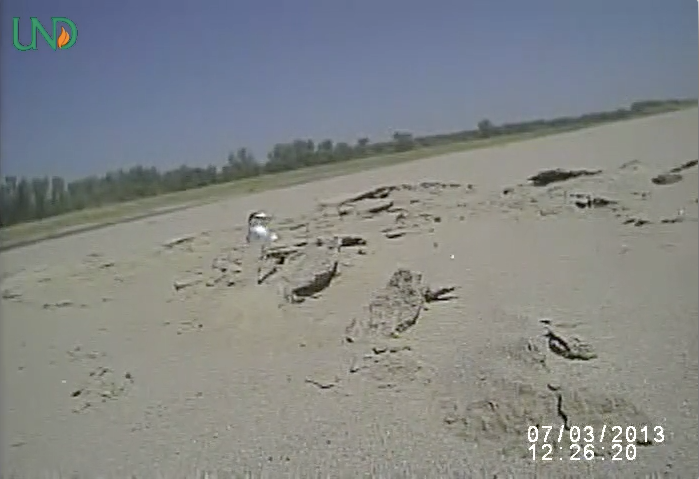
\includegraphics[width=2.9in]{sample_test_frame}
\label{fig:test_frame}}
\hfil
\subfloat[Sample II]{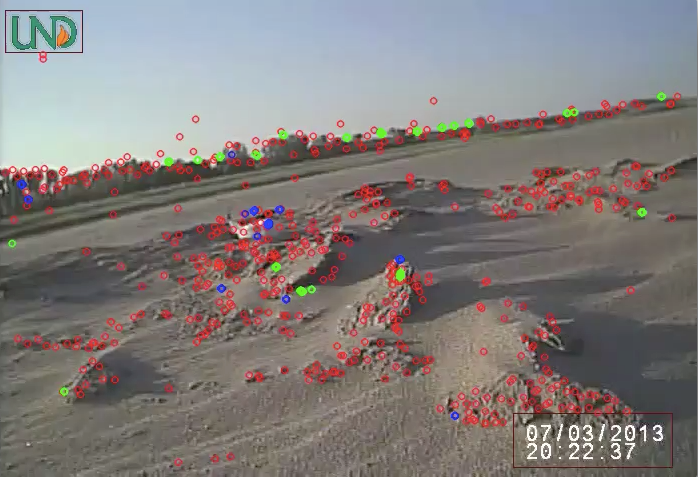
\includegraphics[width=2.9in]{sample_test_begin}
\label{fig:begin_test_video}}
\hfil
\subfloat[Sample III]{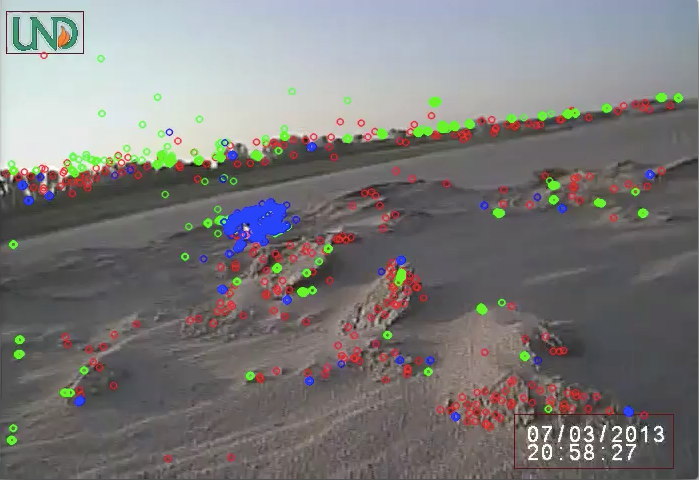
\includegraphics[width=2.9in]{sample_test_end}
\label{fig:end_test_video}}
\caption{These samples show show the progression of feature collection and classification on a Tern nest. We see a frame with no feature overlay (\ref{fig:test_frame}), a frame with a few features overlaid at the beginning of the video (\ref{fig:begin_test_video}), and a frame with all the features from the video overlaid (\ref{fig:end_test_video}). Feature descriptors used for training are shown as blue circles (cumulative), additional positively classified descriptors are shown as green green circles (cumulative), and red circles indicate negatively classified descriptors (non-cumulative). Red boxes indicate regions of the video excluded from the feature detection algorithm.}
\label{fig:machine_learning_example}
\end{sidewaysfigure}

Even with a well-trained SVM and acceptable training error, it is difficult to show that the SVM correctly classifies the descriptors from a video. In order to help test the SVM we need to somehow calculate or show that the points classified are accurate in depicting the object of interest. We do this by color coordinating the keypoints from a video by their classification. Positively classified points colored green and negatively classified points colored red. We also color points that closely match the training descriptors as blue in order to determine the accuracy of our training data. Since each frame has a very sporadic number of points accepted depending on the position of the bird or lighting we show the positively classified points (green) and training descriptors (blue) permanently. An example of this can be see in Figure~\ref{fig:machine_learning_example}.


\section{Background Subtraction}
\label{sec:methods_background_subtraction}

The goal of this research is to determine which algorithms can best highlight regions of uncontrolled outdoor video with \emph{interesting} events. This ideally can act as a filter and help scientists focus on segments of video that require their attention and letting them skip less interesting segments of video. The background subtraction methods need to be resistant to noise and handle quick correction of camera lighting problems while still being sensitive enough to detect the motion of a small to medium sized animal with cryptic coloration. The usefulness of these algorithms is sensitive to the number false positives and false negatives. Too many false positives and there many not be a significant length of video that can be classified as \emph{uninteresting}, while too many false negatives may leave many \emph{interesting} events unclassified and unwatched. An example of this is observed when comparing scientists' observations to positive events from the algorithms, as in Figure~\ref{fig:false_positives_example}. An almost continuous stream of false positives can occur when vegetation moves in the wind when the grouse is not even at the nest (see Figure~\ref{fig:false_positives}), but on less windy days we see increased agreement between the two classifications (see Figure~\ref{fig:no_false_positives}).


\begin{sidewaysfigure}[!t]
\centering
\subfloat[Timeline I]{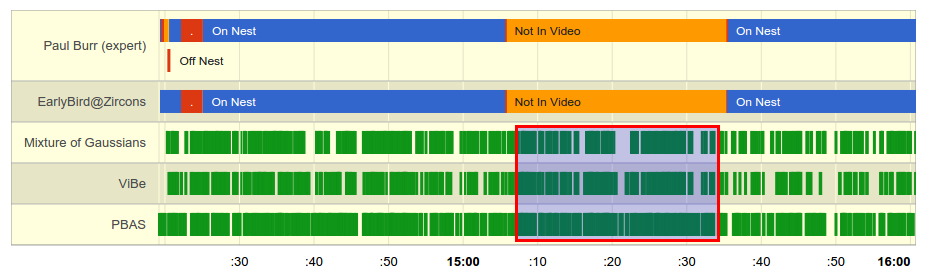
\includegraphics[width=4.2in]{4725_false_positives_grouse}
\label{fig:false_positives}}
\hfil
\subfloat[Timeline II]{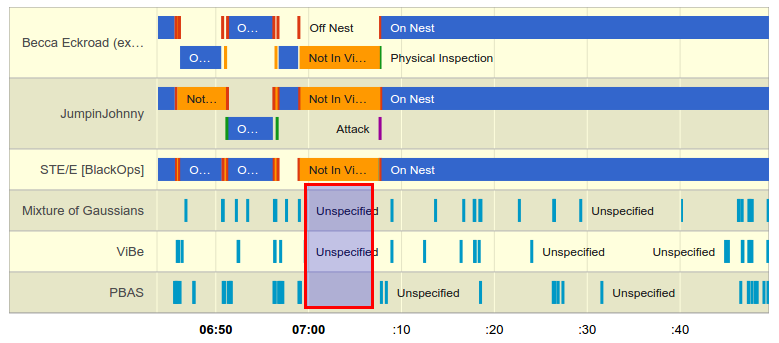
\includegraphics[width=4.2in]{6396_true_positives_grouse}
\label{fig:no_false_positives}}
\caption{Timelines showing the number of false positives in a windy grouse video (\ref{fig:false_positives}) against those in a less windy grouse video (\ref{fig:no_false_positives}). The highlighted regions show time segments from the background subtraction results where there is no bird on the nest. These timelines were created using the Google Charts API~\cite{google_2015_charts} and are easily embedded in the Wildlife@Home user interface.}
\label{fig:false_positives_example}
\end{sidewaysfigure}

Three different algorithms were evaluated for their ability to accurately detect motion in Wildlife@Home's Interior Least Tern, Piping Plover and Sharp-Tailed Grouse video. MOG (see Section~\ref{sec:mog}) was chosen as the baseline for performance, as it is used as a standard for many new background subtraction implementations~\cite{ko_2008_background, piccardi_2004_background, mcivor_2000_background, hofmann_2012_background, elgammal_2000_non, kim_2005_real} and has been successfully used in real world applications~\cite{sen_2004_robust}.


\subsection{Algorithm Modifications}
\label{sec:alg_mods}

Modified versions of ViBe~\cite{van_2014_vibe} and PBAS~\cite{hofmann_2012_background} were implemented and compared to MOG\@. ViBe is a good fit for this problem space as it is non-parametric and can be quickly initialized to prevent a large number of initial false positives. PBAS is an algorithm that adjusts its thresholding and update parameters on a pixel-by-pixel basis. PBAS is also good for this problem, where certain parts of the image are very noisy and at times entire sections of the video are polluted with dynamic lighting changes. PBAS will dynamically increase the foreground classification threshold during portions of a video affected by lighting changes and can learn to ignore regions of a video with large background variance such as in the grouse video (see Figure~\ref{fig:sample_grouse}) where grass movement will span a large area of the video (100's of pixels) and pixel neighborhoods are not enough to detect the movement.

Modifications were made to improve performance on the noisy video and subjects with cryptic coloration. Initialization of ViBe and PBAS were adjusted to be second-frame-ready by adding the minimum number of values to the background model to match the first frame and filling the rest of the background model with values from random locations in the frame. This initialization allows for fast adaptation to subsequent frames if the background has a lot of motion while maintaining the minimum requirement to match the likely similar following frame. An open/close filter was also added to reduce foreground detection noise in the output mask. The mathematical morphology removes small unconnected bits of noise while maintaining the larger connected regions. This prevents many false detections due to video compression and camera induced noise. Depending on the video resolution filter size, this may be adjusted accordingly. Finally, in order to improve detection of birds, we use the convex hull of any connected foreground regions as the foreground mask. Since much of the birds are a similar color to their environment, generally only small areas are detected such as the head, tail feathers, and shadow, and much of the body can remain missing or segmented. The addition of a convex hull to connected foreground regions highlights bird movements and increases algorithm confidence. The convex hull may also be used in the future to detect extreme lighting changes since this will also emphasize large scene changes.


\subsection{Event Calculation}
\label{sec:event_calc}

The conversion from the foreground mask to calculated events is done with time-series analysis. An event is defined as a specified video segment marked with a start and an end time. Foreground pixel counts are taken as a series of data points, and these are smoothed by using an exponential moving average. This further reduces detection noise and sporadic peaks. Once the data is smoothed its mean ($\mu$) and standard deviation ($\sigma$) are calculated and used to determine which frames have more than $3\sigma$ foreground pixels using the inequality in Equation~\ref{eq:outliers}. If this is the case, it is marked as a significant event, otherwise it is ignored. Experimentation can be done to determine a good threshold for the standard deviation.

The equation for the exponential moving average is:

\begin{equation}
    m_t = \alpha \cdot x_t + (1-\alpha) \cdot m_{t-1}
    \label{eq:exponential_moving_average}
\end{equation}

where $m_t$ is the mean at time unit $t$, $x_t$ is the number of foreground pixels at time $t$, and $\alpha$ is the weighted decrease or learning rate. As $\alpha \to 1$ the new data is more heavily weighted. An example this time-series data compared to when scientist marked events occurred can be seen in Figure~\ref{fig:correlation_example}.

The calculation of significant foreground events is done using the following threshold inequality:

\begin{equation}
    x_t > \mu + 3\sigma
    \label{eq:outliers}
\end{equation}

This threshold is a good indication of foreground activity even when the video has a moderate amount of noise since noisy regions are either smoothed or taken into consideration in the time-series mean. The calculated foreground activity can then be compared to scientists to determine algorithm accuracy, as shown in Figure~\ref{fig:false_positives_example}. By calculating events from regions with an abnormal amount of foreground pixels, a measure for the amount of foreground activity taking place is provided. This activity can then be compared to scientists to determine the accuracy of each background subtraction algorithm as shown in Figures~\ref{fig:false_positives_example} and~\ref{fig:correlation_example}.

An example of the correlation between background subtraction events and scientist observed events can be see in Figure~\ref{fig:correlation_example}. The arrows indicate human observed events in comparison with the time-series for each of the three algorithms. The data in these two examples are highly correlated with little noise and very few false detections. It can also be observed that PBAS is very quick to adapt to changes while ViBe has the largest detection emphasis among the three algorithms.

\begin{sidewaysfigure}[!t]
\centering
\subfloat[Sample I]{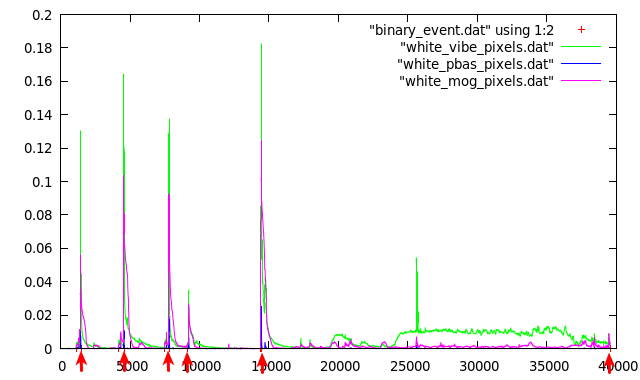
\includegraphics[width=4.3in]{6396_event_correlation}
\label{fig:event_correlation_1}}
\hfil
\subfloat[Sample II]{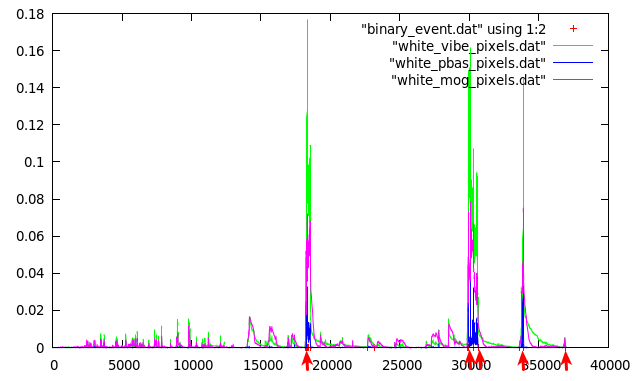
\includegraphics[width=4.3in]{6397_event_correlation}
\label{fig:event_correlation_2}}
\caption{Example of event and foreground pixel count correlation. Red arrows indicate a scientist observed event and lines indicate foreground pixel count for each algorithm.}
\label{fig:correlation_example}
\end{sidewaysfigure}

